\begin{center}
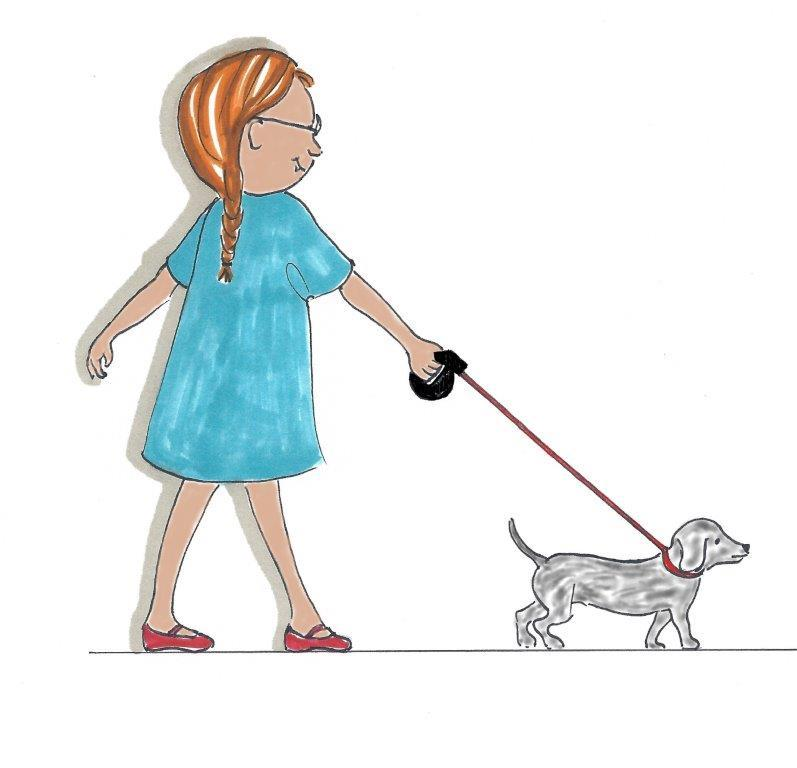
\includegraphics[width=0.4\textwidth]{content/3/chapter5/images/3.png}\\
Cippi在遛狗
\end{center}

std::span表示一个对象,该对象引用一个连续的对象序列。std::span有时也称为视图,其不是底层数据的所有者。这个连续的对象序列可以是一个普通的C数组、有长度信息的指针、std::array、std::vector或std::string。

std::span可以具有静态范围或动态范围。默认情况下,std::span有一个动态范围:

\begin{lstlisting}[style=styleCXX]
template <typename T, std::size_t Extent = std::dynamic_extent>
class span;
\end{lstlisting}

\subsubsubsection{5.2.1\hspace{0.2cm}静态范围与动态范围}

std::span有一个静态范围时,其大小在编译时已知,并且是类型:std::span<T, size>的一部分。因此,其实现只需要一个指向连续对象序列的第一个元素的指针。

具有动态范围的std::span,由指向第一个元素的指针和连续对象序列的长度组成,但长度信息不是类型std::span<T>的一部分。

staticDynamicExtentSpan.cpp展示了这两种视图之间的区别。

\begin{lstlisting}[style=styleCXX]
// staticDynamicExtentSpan.cpp

#include <iostream>
 #include <span>
 #include <vector>

void printMe(std::span<int> container) {
	
	std::cout << "container.size(): " << container.size() << '\n';
	for (auto e : container) std::cout << e << ' ';
	std::cout << "\n\n";
}

int main() {

	std::cout << '\n';
	
	std::vector myVec1{1, 2, 3, 4, 5};
	std::vector myVec2{6, 7, 8, 9};
	
	std::span<int> dynamicSpan(myVec1);
	std::span<int, 4> staticSpan(myVec2);
	
	printMe(dynamicSpan);
	printMe(staticSpan); // implicitly converted into a dynamic span
	
	// staticSpan = dynamicSpan; ERROR
	dynamicSpan = staticSpan;
	
	printMe(staticSpan);
	
	std::cout << '\n';

}
\end{lstlisting}

dynamicSpan(第21行)有一个动态范围,而staticSpan(第22行)有一个静态范围。两个std::span都在printMe函数中返回它们的长度(第9行)。具有动态范围的std::span可以赋值给具有静态范围的std::span,但不能反过来。第27行会导致错误,而第7、25和28行是可以工作的。

\begin{center}
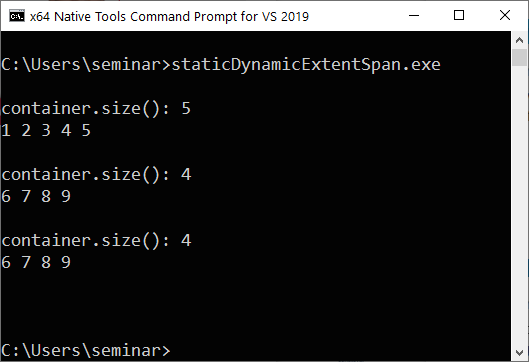
\includegraphics[width=0.6\textwidth]{content/3/chapter5/images/4.png}\\
std::span的静态范围与动态范围
\end{center}

使用std::span<T>的重要原因是,若将普通C数组\href{https://en.cppreference.com/w/cpp/types/decay}{退化}成指针,那么长度信息就会丢失。这种退化是C/C++中出现错误的原因之一。

\subsubsubsection{5.2.2\hspace{0.2cm}自行推断连续对象序列的长度}

与C数组相反,std::span<T>可以自行推断对象连续序列的长度。

\begin{lstlisting}[style=styleCXX]
// printSpan.cpp

#include <iostream>
#include <vector>
#include <array>
#include <span>

void printMe(std::span<int> container) {

	std::cout << "container.size(): " << container.size() << '\n';
	for (auto e : container) std::cout << e << ' ';
	std::cout << "\n\n";
}

int main() {

	std::cout << '\n';
	
	int arr[]{1, 2, 3, 4};
	printMe(arr);
	
	std::vector vec{1, 2, 3, 4, 5};
	printMe(vec);
	
	std::array arr2{1, 2, 3, 4, 5, 6};
	printMe(arr2);

}
\end{lstlisting}

C-array(第19行)、std::vector(第22行)和std::array(第25行)元素类型都是int,所以std::span使用int类型的特化。这个简单的例子中,还有一些更有趣的东西。对于每个容器,std::span可以推断其长度(第10行)。

\begin{center}
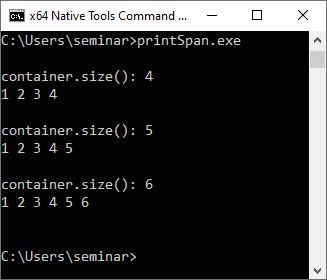
\includegraphics[width=0.4\textwidth]{content/3/chapter5/images/5.png}\\
\end{center}

创建std::span的方法有很多。

\subsubsubsection{5.2.3\hspace{0.2cm}用指针和长度来创建std::span}

可以用指针和内存长度来创建std::span。

\begin{lstlisting}[style=styleCXX]
// createSpan.cpp

#include <algorithm>
#include <iostream>
#include <span>
#include <vector>

int main() {
	
	std::cout << '\n';
	std::cout << std::boolalpha;
	
	std::vector myVec{1, 2, 3, 4, 5};
	
	std::span mySpan1{myVec};
	std::span mySpan2{myVec.data(), myVec.size()};
	
	bool spansEqual = std::equal(mySpan1.begin(), mySpan1.end(),
	                             mySpan2.begin(), mySpan2.end());
	
	std::cout << "mySpan1 == mySpan2: " << spansEqual << '\n';
	
	std::cout << '\n';

}
\end{lstlisting}

由std::vector创建的mySpan1(第15行)和由指针和长度创建的mySpan2(第16行)相同(第21行)。

\begin{center}
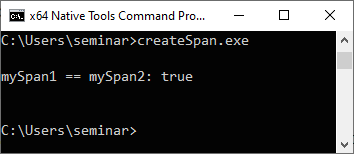
\includegraphics[width=0.5\textwidth]{content/3/chapter5/images/6.png}\\
用指针和长度值来创建std::span
\end{center}

\begin{tcolorbox}[breakable,enhanced jigsaw,colback=red!5!white,colframe=red!75!black,title={std::span既不是std::string\_view也不是视图}]
	
您可能还记得std::span有时会认为是视图,但不要将std::span与范围库中的视图或\href{https://www.modernescpp.com/index.php/c-17-what-s-new-in-the-library}{std::string\_view}混淆。

\hspace*{\fill} \\ %插入空行
范围库中的视图可以对特定范围内的元素执行一些操作。而视图不拥有数据,其复制、移动和赋值的时间成本固定。std::span和std::string\_view虽不是视图,但也可以处理字符串。

\hspace*{\fill} \\ %插入空行
std::span和std::string\_view的主要区别是,std::span可以修改其引用的对象。
\end{tcolorbox}
	
\subsubsubsection{5.2.4\hspace{0.2cm}修改引用对象}

可以修改整个span,也可以只修改子span。修改span时,也会修改引用的对象。

下面的代码展示了如何使用子span来修改std::vector中引用的对象。

\begin{lstlisting}[style=styleCXX]
// spanTransform.cpp

#include <algorithm>
 #include <iostream>
 #include <vector>
 #include <span>

void printMe(std::span<int> container) {
	
	 std::cout << "container.size(): " << container.size() << '\n';
	 for (auto e : container) std::cout << e << ' ';
	 std::cout << "\n\n";
}

int main() {

	std::cout << '\n';
	
	std::vector vec{1, 2, 3, 4, 5, 6, 7, 8, 9, 10};
	printMe(vec);
	
	std::span span1(vec);
	std::span span2{span1.subspan(1, span1.size() - 2)};
	
	
	std::transform(span2.begin(), span2.end(),
	               span2.begin(),
	               [](int i){ return i * i; });
	
	
	printMe(vec);
	printMe(span1);

}
\end{lstlisting}

span1引用std::vector vec(第22行)。相反,span2只引用底层vec的元素,不包括第一个和最后一个元素(第23行)。所以,只对这些元素进行平方的映射(第26行)。

\begin{center}
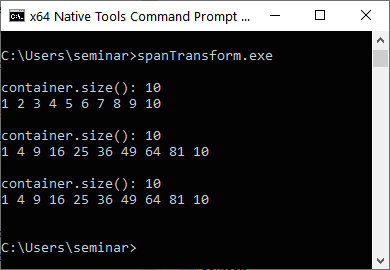
\includegraphics[width=0.5\textwidth]{content/3/chapter5/images/7.png}\\
修改std::span的引用对象
\end{center}

其实,有很多方便的函数可以处理std::span的元素。

\subsubsubsection{5.2.5\hspace{0.2cm}处理std::span的元素}

下表给出了用于引用std::span元素的接口。

\begin{center}
std::span spse的接口
\end{center}

\begin{table}[H]
\centering
\begin{tabular}{ll}
接口         & 描述                                         \\ \hline
sp.front()       & 访问第一个元素。                           \\ \hline
sp.back()        & 访问最后一个元素。                            \\ \hline
sp{[}i{]}        & 访问第i个元素。                            \\ \hline
sp.data()        & 返回一个指向序列开头的指针。 \\ \hline
sp.size()        & 返回元素的个数。     \\ \hline
sp.size\_bytes() & 以字节为单位返回序列的大小。          \\ \hline
sp.empty()       & 若为空,则返回true。              \\ \hline
\begin{tabular}[c]{@{}l@{}}sp.first\textless{}count\textgreater{}()\\ sp.frist(count)\end{tabular} &
返回由序列前count个元素组成的子span。 \\ \hline
\begin{tabular}[c]{@{}l@{}}sp.last\textless{}count\textgreater{}()\\ sp.last(count)\end{tabular} &
返回由序列后count个元素组成的子span。 \\ \hline
\begin{tabular}[c]{@{}l@{}}sp.subspan\textless{}first, count\textgreater{}()\\ sp.subspan(first, count)\end{tabular} &
返回由first之后的count个元素组成的子span。 \\ \hline
\end{tabular}
\end{table}

subspan.cpp展示了成员函数subspan的用法。

\begin{lstlisting}[style=styleCXX]
// subspan.cpp

#include <iostream>
#include <numeric>
#include <span>
#include <vector>

int main() {

	std::cout << '\n';
	
	std::vector<int> myVec(20);
	std::iota(myVec.begin(), myVec.end(), 0);
	for (auto v: myVec) std::cout << v << " ";
	
	std::cout << "\n\n";
	
	std::span<int> mySpan(myVec);
	auto length = mySpan.size();
	
	std::size_t count = 5;
	for (std::size_t first = 0; first <= (length - count); first += count ) {
		for (auto ele: mySpan.subspan(first, count)) std::cout << ele << " ";
		std::cout << '\n';
	}

}
\end{lstlisting}

第13行使用算法\href{https://en.cppreference.com/w/cpp/algorithm/iota}{std::iota}用从0到19的所有数字填充vector(第13行),这个vector用于初始化std::span(第18行)。最后,for循环(第22行)使用subspan函数创建子span,从第一个开始直到使用mySpan为止,子span都包含count个元素。

\begin{center}
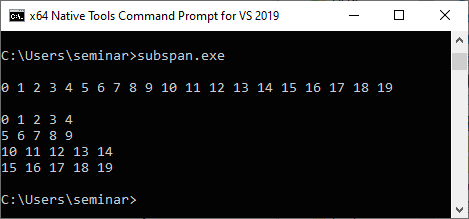
\includegraphics[width=0.6\textwidth]{content/3/chapter5/images/8.png}\\
使用成员函数subspan
\end{center}

Kilian Henneberger给我说了一个std::span的特殊用例,可修改元素的常量范围。

\subsubsubsection{5.2.6\hspace{0.2cm}可修改元素的常量范围}

简单起见,我将std::vector和std::span命名为一个范围。与std::string类似,std::vector对可修改元素的可修改范围进行建模:std::vector<T>。当把std::vector声明为const时,范围模型就表示常量对象的常量范围:不能对可修改元素的常量范围进行建模。std::span对一个常量范围的可修改对象建模:std::span<T>。下表强调了(常量/可修改)范围和(常量/可修改)元素的变化。

\begin{center}
(常量/可修改)元素的(常量/可修改)范围
\end{center}

\begin{table}[H]
\centering
\begin{tabular}{lll}
&
\textbf{可修改的元素} &
\textbf{常量元素} \\ \hline
\textbf{可修改的范围} &
std::vector\textless{}T\textgreater{} &
\\ \hline
\textbf{常量范围} &
std::span\textless{}T\textgreater{} &
\begin{tabular}[c]{@{}l@{}}const std::vector\textless{}T\textgreater\\ std::span\textless{}const T\textgreater{}\end{tabular}
\end{tabular}
\end{table}

constRangeModifiableElements.cpp展示了每种组合。

\begin{lstlisting}[style=styleCXX]
// constRangeModifiableElements.cpp

#include <iostream>
#include <span>
#include <vector>

void printMe(std::span<int> container) {

	std::cout << "container.size(): " << container.size() << '\n';
	for (auto e : container) std::cout << e << ' ';
	std::cout << "\n\n";
}

int main() {

	std::cout << '\n';
	
	std::vector<int> origVec{1, 2, 2, 4, 5};
	
	// Modifiable range of modifiable elements
	std::vector<int> dynamVec = origVec;
	dynamVec[2] = 3;
	dynamVec.push_back(6);
	printMe(dynamVec);
	
	// Constant range of constant elements
	const std::vector<int> constVec = origVec;
	// constVec[2] = 3; ERROR
	// constVec.push_back(6); ERROR
	std::span<const int> constSpan(origVec);
	// constSpan[2] = 3; ERROR
	
	// Constant range of modifiable elements
	std::span<int> dynamSpan{origVec};
	dynamSpan[2] = 3;
	printMe(dynamSpan);
	
	std::cout << '\n';

}
\end{lstlisting}

vector dynamVec(第21行)是可修改元素的可修改范围。这个观察结果不适用于vector constVec(第27行),constVec不能改变元素的多少,constSpan(第30行)的行为也一样。dynamSpan为常量范围的可修改元素提供了一种方式。

\begin{center}
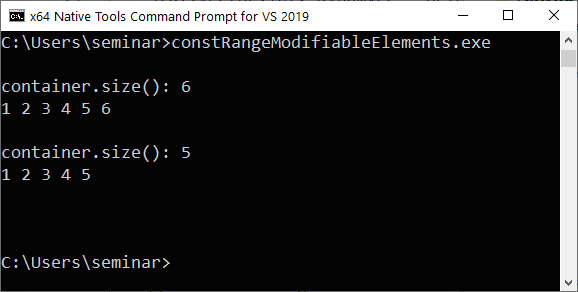
\includegraphics[width=0.6\textwidth]{content/3/chapter5/images/9.png}\\
(常量/可修改)元素的(常量/可修改)范围
\end{center}

\begin{tcolorbox}[breakable,enhanced jigsaw,colback=mygreen!5!white,colframe=mygreen!75!black,title={总结}]

\begin{itemize}
\item 
std::span是一个引用连续对象序列的对象。std::span也称为视图,从来不是数据的所有者,因此不分配内存。对象的连续序列可以是一个C数组、带内存长度的指针、std::array、std::vector或std::string。

\item 
与C数组相反,std::span可以自动推断其引用对象序列的长度。

\item 
std::span修改其元素时,也会修改其引用的对象。
\end{itemize}

\end{tcolorbox}

\newpage








